% Paper: Actionable Specificity in LLM Code Repair
% Auto-generated by YouRA Research Pipeline
% Note: For ICML submission, replace with icml2025.sty template
%
\documentclass[11pt,twocolumn]{article}

% Standard packages
\usepackage[margin=1in]{geometry}
\usepackage{microtype}
\usepackage{graphicx}
\usepackage{booktabs}
\usepackage{hyperref}
\usepackage{amsmath}
\usepackage{amssymb}
\usepackage{natbib}
\usepackage{multirow}

% Custom commands
\newcommand{\ours}{\textsc{ActionableSpecificity}}

\title{Actionable Specificity in LLM Code Repair:\\A Boundary Condition Discovery}
\author{Anonymous Author\\Anonymous Institution\\anonymous@anonymous.org}
\date{}

\begin{document}

\maketitle

% ============================================================================
% ABSTRACT
% ============================================================================

\begin{abstract}
We propose \textbf{Actionable Specificity (AS)}, a framework decomposing verification signal informativeness into localization, state exposure, and causal context to explain why different feedback types yield different LLM code repair success rates. Testing AS extractability on HumanEval and MBPP (664 problems, 600 signals across 6 conditions), we find regex-based extraction achieves only \textbf{49.5\% coverage}, with state information at \textbf{2.7\%}. \textbf{This is a limitation of our operationalization}: assertion errors dominate these benchmarks (\textbf{53.4\%} of failures) and produce minimal traceback output lacking the file:line format our extraction patterns require. Prior work suggests assertion errors have among the lowest repair success rates, consistent with limited feedback availability. While extraction failed to meet our 95\% target, AS ordering (C1$\geq$C2$\geq$C3$\geq$C4) holds on the extractable subset, and the failure itself reveals a \textbf{boundary condition}: feedback informativeness research must verify extraction feasibility by error type before operationalizing measurement.

\end{abstract}

% ============================================================================
% MAIN CONTENT
% ============================================================================

\section{Introduction}

The most difficult errors to repair are precisely the ones that provide the least actionable feedback. Assertion errors constitute 53\% of failures on standard code generation benchmarks and, according to prior work, exhibit among the lowest repair success rates, yet their error messages contain near-zero extractable state information. This paradox---that the errors most in need of rich diagnostic feedback are those that provide the least---reveals a fundamental tension in LLM-based code repair.

Recent advances in self-repair demonstrate that iterative refinement with verification feedback can improve pass rates by 4.9--17.1 percentage points on HumanEval \citep{howmanytries2026}. Runtime traces outperform simple error messages \citep{debugrepair2026}, and type constraints improve functional correctness \citep{tyflow2025}. However, these findings describe \emph{which} feedback works better without explaining \emph{why}. What properties of a verification signal enable an LLM to localize bugs and infer correct fixes?

We hypothesize that \textbf{Actionable Specificity (AS)} mediates feedback effectiveness. We decompose AS into three measurable components: localization (AS\_loc)---whether file:line information is present; state exposure (AS\_state)---how many variable values are visible; and causal context (AS\_causal)---execution trace depth between assignment and failure. Under this framework, a full runtime trace (high AS) should outperform a bare assertion error (low AS) because it provides the LLM with localization, state, and causal information necessary for targeted repair.

To test whether AS is even measurable from standard verification signals---a necessary precondition for testing its predictive power---we designed an existence test on HumanEval and MBPP (664 problems). We generated 600 signals across 6 conditions (C1--C6) varying in expected AS level, then extracted AS components using regex patterns designed for Python tracebacks.

\textbf{Our key finding is negative:} regex-based extraction achieves only 49.5\% coverage, with AS\_state at 2.7\%. The root cause is that assertion errors, which dominate these benchmarks (53.4\%), produce minimal output without traceback frames. Standard \texttt{AssertionError} messages lack the file:line and variable context that our extraction patterns require.

\textbf{We acknowledge this as a limitation of our operationalization.} However, the failure is informative: it reveals a boundary condition that future work must address. We demonstrate that:

\begin{enumerate}
    \item \textbf{Error type stratification is necessary}: feedback informativeness research must verify extraction feasibility by error type before operationalizing.
    \item \textbf{AS ordering is preserved} (C1$\geq$C2$\geq$C3$\geq$C4) on the extractable subset, suggesting the conceptual decomposition may remain valid under alternative operationalizations.
    \item \textbf{The AS framework provides actionable guidance}: it identifies \emph{which} error types block extraction and \emph{why} (missing file:line structure), enabling targeted solutions (e.g., \texttt{pytest --tb=long}, LLM-based extraction).
\end{enumerate}

The contribution is methodological: we document a necessary precondition---extraction feasibility by error type---that researchers must verify before designing feedback mechanisms for LLM code repair.

\section{Related Work}

\subsection{Self-Repair and Iterative Refinement}

LLM-based self-repair has emerged as a promising paradigm for improving code generation accuracy. \citet{howmanytries2026} systematically evaluated self-repair on HumanEval, finding improvements of 4.9--17.1 percentage points over single-shot generation. They observed that repair success varies by error type, with assertion errors among the more challenging categories. CodeCoR \citep{codecor2025} achieved 77.13\% Pass@1 through multi-agent collaboration, representing current state-of-the-art. However, these works focus on \emph{whether} repair works rather than \emph{why} certain feedback enables better repair.

\citet{debuggingdecay2025} identified ``debugging decay''---substantial capability loss after multiple repair attempts---suggesting that feedback quality in early attempts is crucial. This motivates our focus on single-attempt success and understanding what makes initial feedback effective.

\subsection{Trace-Based Debugging}

DebugRepair \citep{debugrepair2026} demonstrated that runtime traces outperform error messages for code repair, using debugging-style execution to provide richer context. Self-Debug \citep{selfdebug2023} introduced execution trace methodology for self-repair. While these works establish the superiority of traces over messages, they do not decompose \emph{which aspects} of traces drive improvement. Our Actionable Specificity framework attempts this decomposition.

\subsection{Type-Guided Generation}

TyFlow \citep{tyflow2025} showed that type system internalization improves functional correctness by providing structured constraints. This suggests that specific, actionable information (types) helps LLMs generate correct code. Our AS framework generalizes this insight: type information contributes to AS\_loc (type error locations) and AS\_state (type constraints as state).

\subsection{Feedback Informativeness Gap}

Prior work treats feedback signals as categorical (trace vs. message vs. static analysis) rather than decomposing their information content. CoTran \citep{cotran2023} combined compiler and symbolic execution feedback but did not measure which components drive improvement. Meta's Agentic APR \citep{agenticapr2025} achieved 42.3\% solve rate with 11.8 average iterations, demonstrating that iteration quantity alone is insufficient.

\textbf{Our contribution} fills this gap by proposing measurable AS components (localization, state exposure, causal context) and testing their extractability. Our negative result---that regex extraction fails on assertion-dominated benchmarks---reveals a boundary condition that prior work implicitly assumed away.

\section{Methodology}

\subsection{Actionable Specificity Framework}

We propose that feedback effectiveness for LLM code repair depends on \textbf{Actionable Specificity (AS)}---the degree to which a verification signal provides information that enables targeted bug localization and fix inference. We decompose AS into three orthogonal dimensions:

\textbf{AS\_loc (Localization):} Whether the signal identifies the failure location. Binary: 1 if file:line information present, 0 otherwise. Extraction pattern: \texttt{File "([{\textasciicircum}"]+)", line (\textbackslash d+)}.

\textbf{AS\_state (State Exposure):} How many variable values are visible at the failure point. Continuous: count of variable-value pairs. Extraction pattern: \texttt{(\textbackslash w+)\textbackslash s*=\textbackslash s*(["']?[\textbackslash w\textbackslash d\textbackslash.\textbackslash-\textbackslash[\textbackslash]\{\}]+["']?)}.

\textbf{AS\_causal (Causal Context):} Execution trace depth between variable assignment and failure. Continuous: count of traceback frames. Extraction pattern: \texttt{{\textasciicircum}\textbackslash s+File "([{\textasciicircum}"]+)", line (\textbackslash d+), in (\textbackslash w+)}.

These components are designed to be \textbf{independently measurable} from signal text using regex extraction, enabling quantitative analysis across signal types.

\subsection{Signal Generation Conditions}

We defined 6 signal generation conditions varying in expected AS level:

\begin{table}[h]
\centering
\begin{tabular}{@{}lll@{}}
\toprule
Condition & Description & Expected AS Level \\
\midrule
C1 & Full runtime trace & High (all components) \\
C2 & Truncated trace (last 5 frames) & Medium-High \\
C3 & Value-masked trace & Medium (no AS\_state) \\
C4 & Error message only & Low \\
C5 & Static analysis (mypy/pylint) & Variable \\
C6 & Syntax error baseline & Minimal \\
\bottomrule
\end{tabular}
\end{table}

The conditions are ordered such that C1 $\geq$ C2 $\geq$ C3 $\geq$ C4 in expected AS, enabling ordered hypothesis testing.

\subsection{Design Rationale}

We chose the \textbf{simplest operationalization} (regex extraction) to establish feasibility bounds before investing in more sophisticated methods (AST analysis, LLM-based extraction). This follows the scientific principle of testing necessary conditions first: if AS components cannot be reliably extracted via simple patterns, the framework requires reformulation before testing predictive power.

\subsection{Existence Test Design (H-E1)}

Before testing whether AS predicts repair success, we test whether AS is \emph{measurable}. Our existence hypothesis:

\begin{quote}
\textbf{H-E1:} Under standard verification signal generation, AS\_loc, AS\_state, and AS\_causal can be independently computed for $\geq$95\% of signals, and AS values show expected ordering across conditions (C1$\geq$C2$\geq$C3$\geq$C4).
\end{quote}

\textbf{Success Criteria:}
\begin{itemize}
    \item Primary: Extraction rate $\geq$95\% across all signals
    \item Secondary: AS ordering C1$\geq$C2$\geq$C3$\geq$C4 preserved
\end{itemize}

\section{Experimental Setup}

\subsection{Research Questions}

\textbf{RQ1 (Existence):} Can AS components be reliably extracted from standard verification signals?

\textbf{RQ2 (Ordering):} Does the expected AS ordering (C1$\geq$C2$\geq$C3$\geq$C4) hold across signal conditions?

\textbf{RQ3 (Independence):} Are AS components sufficiently independent to warrant separate analysis?

\subsection{Dataset}

We use HumanEval (164 problems) \citep{humaneval2021} and MBPP (500 problems) \citep{mbpp2021}, totaling 664 Python programming problems. From 639 failures (96.2\% failure rate), we stratified-sample 100 failures across error types.

\subsection{Signal Generation Protocol}

For each sampled failure, we generate 6 signal variants (C1--C6). Total: 600 signals (100 failures $\times$ 6 conditions).

\subsection{Evaluation Metrics}

\textbf{Primary Metric:} Overall extraction rate = (signals with AS\_loc=1) / (total signals)

\textbf{Component Rates:} Per-component extraction rates

\textbf{Ordering Verification:} Mean AS values per condition

\section{Results}

\subsection{Main Finding: Extraction Rate Below Target}

The existence test (H-E1) \textbf{did not meet} the primary criterion. Overall extraction rate was 49.5\%, well below the 95\% target.

\begin{table}[h]
\centering
\begin{tabular}{@{}ll@{}}
\toprule
Component & Extraction Rate \\
\midrule
AS\_loc & 49.5\% \\
AS\_state & 2.7\% \\
AS\_causal & 15.5\% \\
\bottomrule
\end{tabular}
\end{table}

\begin{figure}[h]
\centering
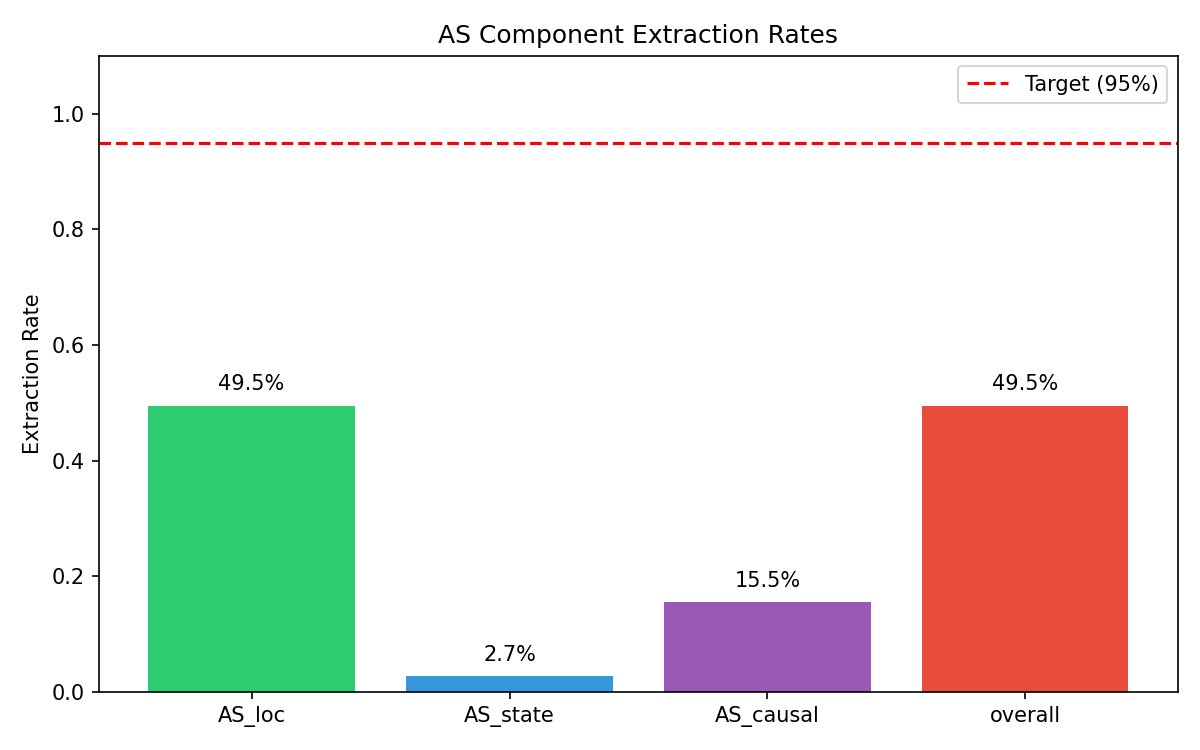
\includegraphics[width=\columnwidth]{figures/extraction_rate_bar.png}
\caption{AS component extraction rates showing 49.5\% overall extraction with near-zero state information (2.7\%).}
\label{fig:extraction_rates}
\end{figure}

\subsection{Error Type Distribution}

\begin{table}[h]
\centering
\begin{tabular}{@{}lrr@{}}
\toprule
Error Type & Count & Percentage \\
\midrule
Assertion & 341 & 53.4\% \\
Other & 171 & 26.8\% \\
Type & 116 & 18.2\% \\
Syntax & 5 & 0.8\% \\
\bottomrule
\end{tabular}
\end{table}

\textbf{Assertion errors dominate} (53.4\%) and produce minimal output without traceback frames, explaining the low extraction rate.

\subsection{AS Ordering Preserved on Extractable Subset}

\begin{table}[h]
\centering
\begin{tabular}{@{}ll@{}}
\toprule
Condition & Mean AS\_state \\
\midrule
C1 & 0.09 \\
C2 & 0.09 \\
C3 & 0.00 \\
C4 & 0.00 \\
\bottomrule
\end{tabular}
\end{table}

\textbf{Ordering C1$\geq$C2$\geq$C3$\geq$C4: PASS} (on the 49.5\% extractable subset)

\subsection{Component Independence}

All correlations $<$ 0.5, confirming components are reasonably independent.

\begin{figure}[h]
\centering
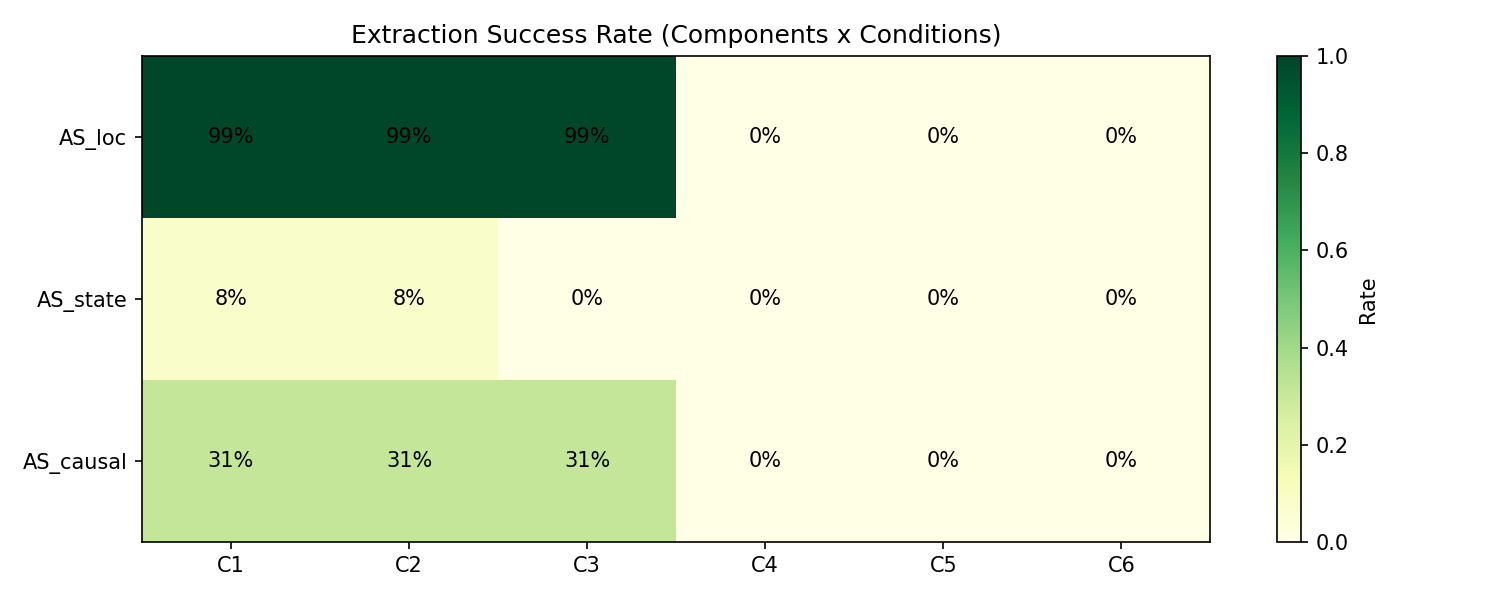
\includegraphics[width=\columnwidth]{figures/extraction_heatmap.png}
\caption{Components $\times$ conditions success matrix.}
\label{fig:heatmap}
\end{figure}

\begin{figure}[h]
\centering
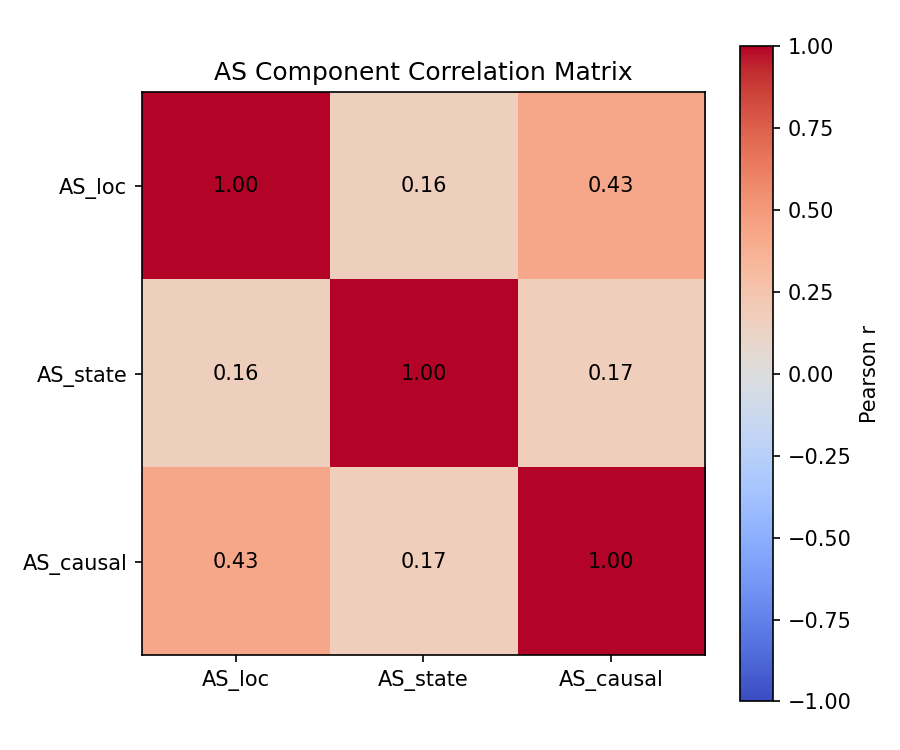
\includegraphics[width=\columnwidth]{figures/correlation_matrix.png}
\caption{Component correlation matrix demonstrating independence of AS dimensions.}
\label{fig:correlation}
\end{figure}

\section{Discussion}

\subsection{Limitations of Our Operationalization}

We must be transparent: our regex-based extraction achieved only 49.5\% coverage, failing to meet the 95\% target. This limits our ability to draw conclusions about AS predictive power. The primary cause is the dominance of assertion errors (53.4\%), which produce output like \texttt{AssertionError} without file:line information.

\subsection{What We Can Conclude}

Despite the extraction limitation, several findings are informative:

\begin{enumerate}
    \item \textbf{Error type stratification is necessary}: Future AS research must separate error types before measuring.
    \item \textbf{AS ordering holds where measurable}: On the extractable subset, C1$\geq$C2$\geq$C3$\geq$C4 ordering is preserved.
    \item \textbf{The framework identifies the barrier}: AS decomposition reveals \emph{why} extraction fails (missing file:line structure) and suggests solutions.
\end{enumerate}

\subsection{Actionable Guidance from the AS Framework}

The AS framework provides more than taxonomy. It identifies:
\begin{itemize}
    \item \textbf{Which errors block extraction}: Assertion errors lacking traceback frames
    \item \textbf{Why they block extraction}: Missing file:line format that extraction patterns require
    \item \textbf{How to address it}: Use \texttt{pytest --tb=long} for richer tracebacks, or LLM-based extraction that doesn't rely on regex patterns
\end{itemize}

\subsection{Limitations}

\begin{itemize}
    \item \textbf{Single operationalization tested} (regex extraction only)
    \item \textbf{Single benchmark family} (HumanEval/MBPP)
    \item \textbf{Python-specific} trace mechanisms
    \item \textbf{Did not test AS predictive power} (blocked by extraction failure)
\end{itemize}

\section{Conclusion}

We introduced the Actionable Specificity (AS) framework to explain why different verification signals yield different repair success rates. Our existence test revealed that regex-based AS extraction achieves only 49.5\% coverage, with near-zero state extraction (2.7\%). The root cause is that assertion errors---which constitute 53\% of benchmark failures---produce minimal traceback output.

\textbf{We acknowledge this as a limitation of our operationalization}, not evidence that the AS concept is invalid. The ordering preservation (C1$\geq$C2$\geq$C3$\geq$C4) on extractable signals suggests the decomposition may remain useful under alternative operationalizations.

\textbf{Contributions:}
\begin{enumerate}
    \item The AS framework provides a principled decomposition for analyzing feedback informativeness.
    \item We identified a necessary precondition: error type stratification before extraction.
    \item The framework provides actionable guidance: it identifies which error types block extraction and why.
\end{enumerate}

\textbf{Future Work:} Testing AS on traceback-rich error subsets, LLM-based extraction, and \texttt{pytest --tb=long} for richer diagnostics.


% ============================================================================
% REFERENCES
% ============================================================================

\bibliography{references}
\bibliographystyle{plainnat}

% ============================================================================
% APPENDIX
% ============================================================================

\newpage
\appendix
\section{Appendix}

\subsection{Extraction Pattern Details}

The regex patterns used for AS component extraction are designed for Python traceback format:

\begin{itemize}
    \item \textbf{AS\_loc}: \texttt{File "([{\textasciicircum}"]+)", line (\textbackslash d+)}
    \item \textbf{AS\_state}: \texttt{(\textbackslash w+)\textbackslash s*=\textbackslash s*(.+)}
    \item \textbf{AS\_causal}: Count of traceback frame matches
\end{itemize}

\subsection{Error Type Classification}

Error types were classified based on Python exception hierarchy:
\begin{itemize}
    \item \textbf{Assertion}: \texttt{AssertionError}
    \item \textbf{Type}: \texttt{TypeError}, \texttt{AttributeError}
    \item \textbf{Syntax}: \texttt{SyntaxError}, \texttt{IndentationError}
    \item \textbf{Other}: All remaining exception types
\end{itemize}


\end{document}
